\documentclass{article}
\usepackage[utf8]{inputenc}
\usepackage{hyperref}
\hypersetup{
colorlinks=true,
    linkcolor=black,
    filecolor=black,      
    urlcolor=blue,
    citecolor=black,
}
\usepackage[letterpaper, portrait, margin=1in]{geometry}
\usepackage{enumitem}
\usepackage{amsmath}
\usepackage{booktabs}
\usepackage{graphicx}
\usepackage{titlesec}

\titleformat{\section}
{\normalfont\Large\bfseries}{\thesection}{1em}{}[{\titlerule[0.8pt]}]
  
\title{Homework 4 \\ Economics 7103}
\author{Ana Mazmishvili}
\date{February 12}
  
\begin{document}
  
\maketitle

\section{Python}

\noindent 1. See figure \ref{fig:trend}

\begin{figure}[h]
    \centering
    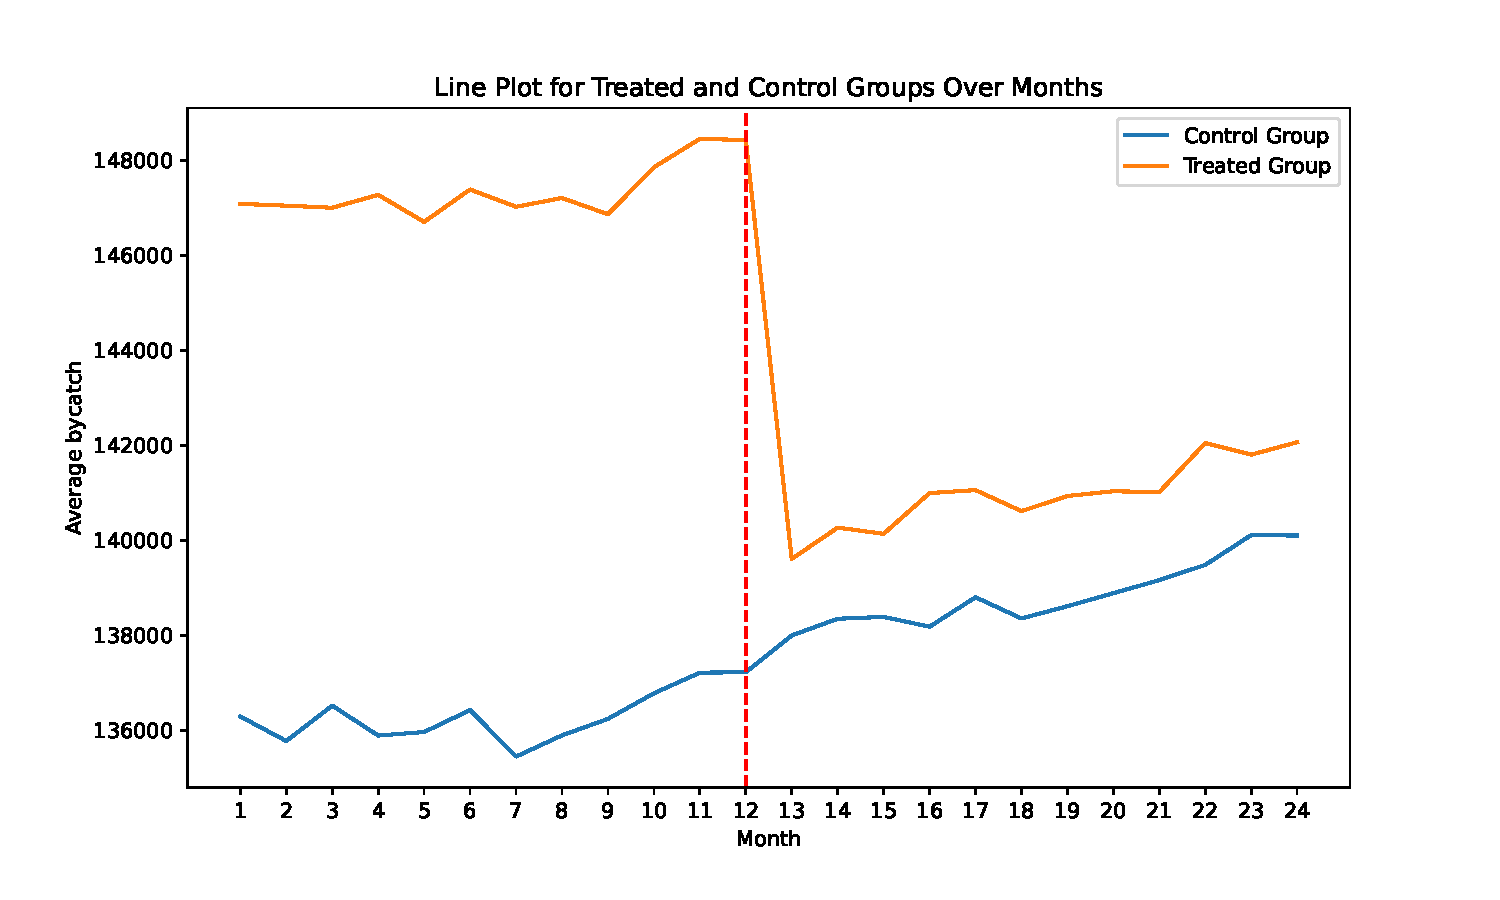
\includegraphics{homework 4/output/figure/trend1.pdf}
    \caption{ Bycatch by month before and after treatment. }
    \label{fig:trend}
\end{figure}

\noindent 2. See table \ref{tab:DID1}

\begin{table}[]
    \centering
    const             136310.169457
treated            11052.449649
post_treatment      2563.075526
trt_posttrt        -8956.783746
dtype: float64

    \caption{DID results}
    \label{tab:DID1}
\end{table}


\noindent 3. Each method produces quite similar results that probably only differ in rounding error:


\noindent 4. See table .  If randomization worked, the simple difference-in-means is an unbiased estimate of the treatment effect.

\section{Stata}

\noindent \textbf{1.a.} I generated firm and month indicator variables and included all of them in the regression. Stata dropped two firm indicator variables and one month indicator variable. The DID estimator is presented in the Table \ref{tab:OLS}. 

\noindent 1.b. After demeaning at the firm level, "firmsize" and "firm" dummy variables were eliminated, but month variable will get negative results after demeaning. I am not sure what we should do with time dummies
\noindent 1.c See table \ref{tab:OLS}

\begin{table}[]
    \centering
    \begin{tabular}{l*{3}{c}}
\hline\hline
                    &\multicolumn{1}{c}{(a)}&\multicolumn{1}{c}{(b)}&\multicolumn{1}{c}{(c)}\\
\hline
Tretment Effect Estimates&    -8085.14&    -8085.14&    -8149.06\\
                    &   (2619.21)&   (2563.92)&   (2489.02)\\
\hline
Method              &OLS with Firm & Month FE&Demeaned OLS with Month FE&Demeaned OLS without Month FE\\
Observations        &        1200&        1200&        1200\\
\hline\hline
\end{tabular}

    \caption{Estimating the DID estimators using OLS regression}
    \label{tab:OLS}
\end{table}




\end{document}